\chapter{Interface de Gerenciamento: RSCADA}
\label{chap:interface-web}

A interface de gerenciamento foi desenvolvida conforme todos os conceitos descritos no Capítulo \ref{chap:sistema-proposto}, o tema utilizado para estilo da página foi desenvolvido pela empresa Colorlib com código-fonte aberto e modificado à critérios do projeto \cite{Concept}. O nome do sistema, RSCADA,  foi constituído da inicial R do nome do autor e o tipo do sistema em questão. Todo o código dos módulos foi programado utilizando a linguagem de programação PHP, com exceção da integração entre o banco de dados e o serviço VerneMQ, responsável pelo protocolo MQTT, teve por base programação LUA e os exemplos de utilização da plataforma disponíveis no Capítulo \ref{chap:resultados} que foram desenvolvidos utilizando C++ com pequenas modificações. Todas as etapas e telas do projeto são explicadas a seguir.

\section{Acesso ao Sistema}
\label{sec:acesso-sistema}
Ao acessar a interface de gerenciamento, é solicitado ao utilizador os dados de acesso, sendo eles: usuário ou e-mail e senha. Na Figura \ref{fig:figura-rscada-1} é apresentada a tela real de acesso do sistema desenvolvido.

        \begin{figure}[!h]
		\Caption{\label{fig:figura-rscada-1} Tela de autenticação da Interface Web.}
		%\centering
		\UFCfig{}{
			\fbox{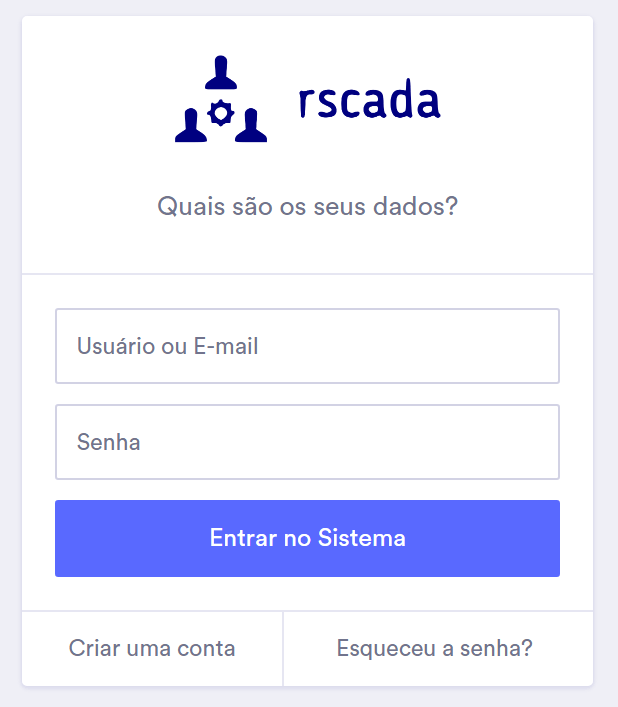
\includegraphics[width=9cm]{figuras/rscada-1.png}}
		}{
			\Fonte{O autor}
		}	
    	\end{figure}

Caso seja um novo utilizador, é fornecido um botão na tela de acesso para criação de novas contas, onde o sistema redirecionará à página de criação de contas e solicitará ao novo usuário: Nome, E-mail, Usuário e Senha, além de uma confirmação de leitura sobre os termos de serviço do RSCADA. Ao submeter o formulário de criação de nova conta, é enviado ao email do usuário, um \textit{link} contendo um código de confirmação da conta para validar o e-mail digitado. A Figura \ref{fig:figura-rscada-2} demonstra a tela de cadastro para novas contas do RSCADA.

        \begin{figure}[!h]
		\Caption{\label{fig:figura-rscada-2} Tela de cadastro para novos usuários.}
		%\centering
		\UFCfig{}{
			\fbox{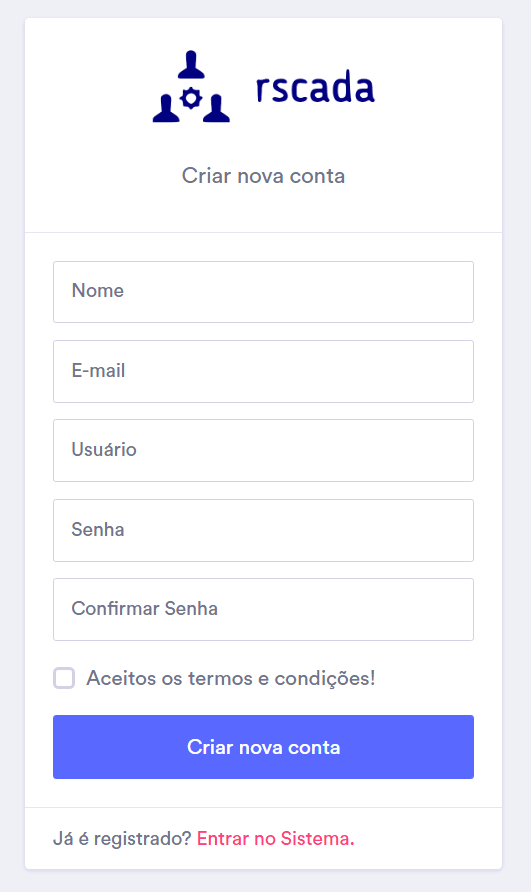
\includegraphics[width=9cm]{figuras/rscada-2.png}}
		}{
			\Fonte{O autor}
		}	
    	\end{figure}

\section{Tela inicial da interface}
\label{sec:tela-inicial}
Devidamente autenticado no sistema, o usuário é redirecionado à tela inicial onde o foco são os projetos cadastrados pertencentes a ele. Informações sobre a quantidade de Clientes associados aos projetos e botões de ações, são disponíveis na página, dentre elas: Novo Projeto, Gerenciamento dos Projetos existentes e Exclusão dos mesmos. Um menu é disponibilizado na lateral esquerda da tela, com os principais atalhos para funções do sistema, como: (i) Minha Conta, onde o usuário poderá alterar detalhes como: E-mail ou Senha, (ii) Meus Projetos, quando necessário retornar à tela inicial dos projetos, (iii) Meus Clientes, para o cadastro de clientes descritos anteriormente como Operadores, que farão uso dos projetos quando desenvolvidos, (iv) Meus Domínios, que o usuário poderá cadastrar o endereço de site o qual os clientes terão acesso ao projeto desenvolvido, (v) Alarmes, para visualizar eventos e alertas de informações que tenham sido inseridas no sistema e que não correspondem aos valores ideiais de funcionamento, entre outros. Nas Figuras \ref{fig:figura-rscada-3} e \ref{fig:figura-rscada-5}, são apresentadas capturas da tela descrita.

        \begin{figure}[!h]
		\Caption{\label{fig:figura-rscada-3} Tela inicial do sistema após autenticação.}
		%\centering
		\UFCfig{}{
			\fbox{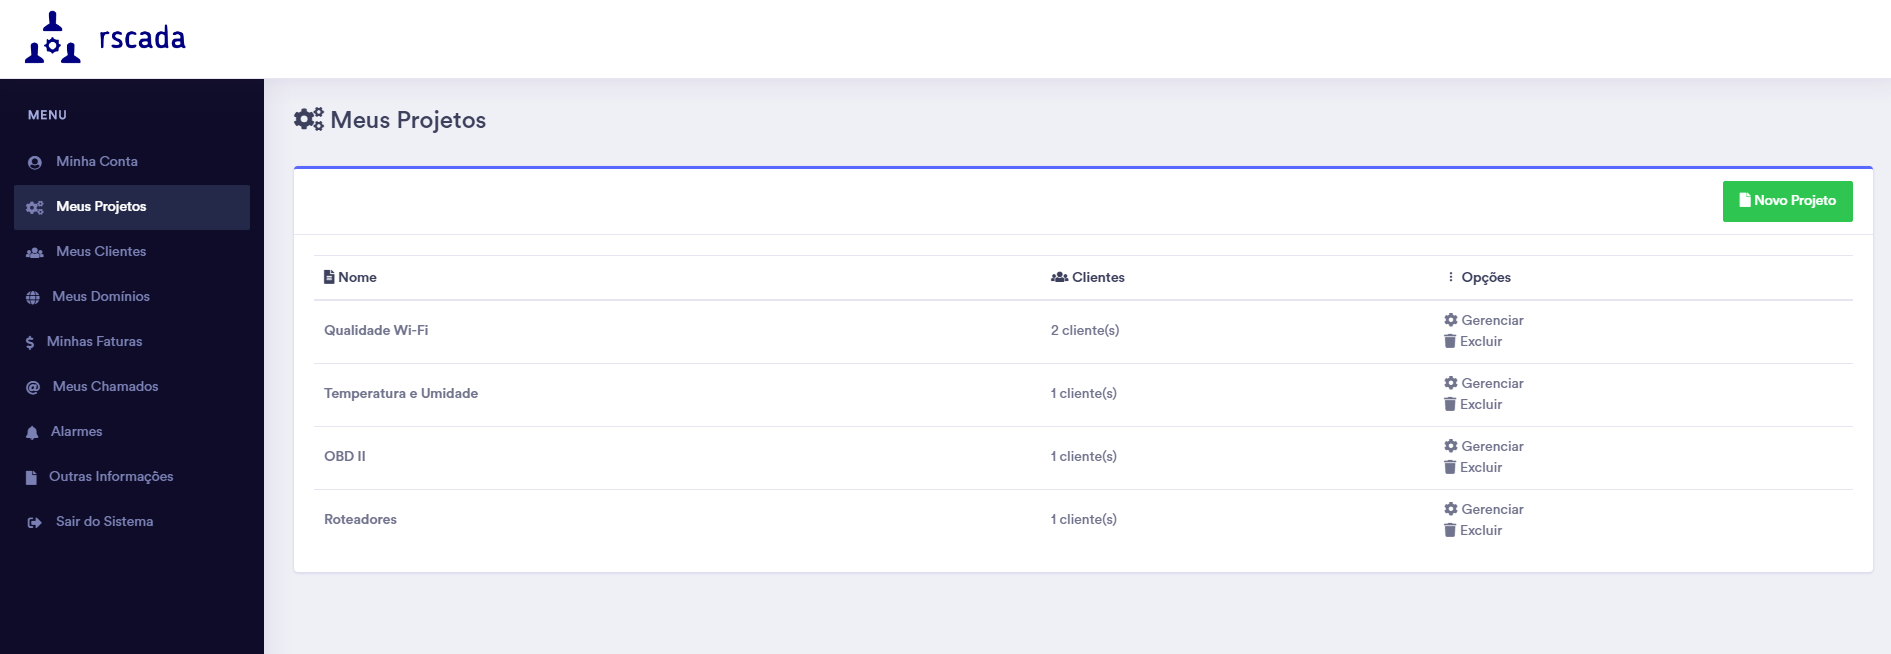
\includegraphics[width=15cm]{figuras/rscada-3.png}}
		}{
			\Fonte{O autor}
		}	
    	\end{figure}
    	
    	\begin{figure}[!h]
		\Caption{\label{fig:figura-rscada-5} Apresentação Geral de todos os projetos cadastrados.}
		%\centering
		\UFCfig{}{
			\fbox{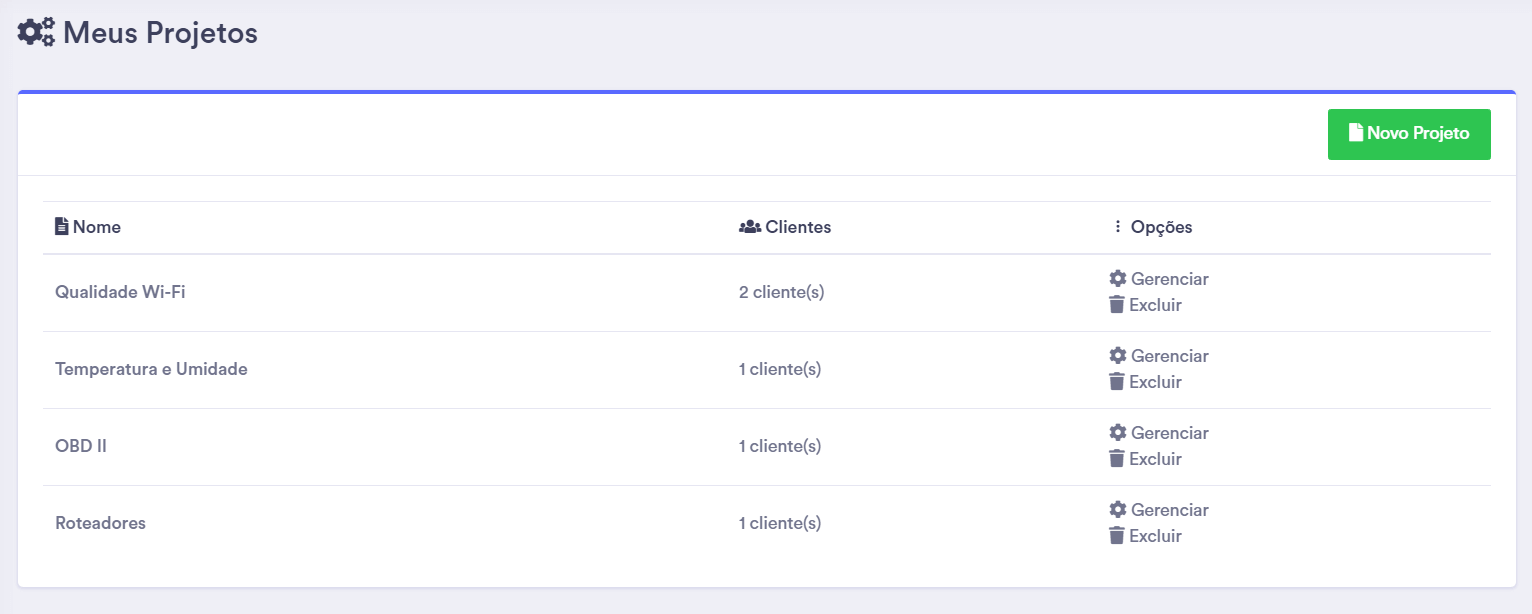
\includegraphics[width=15cm]{figuras/rscada-5.png}}
		}{
			\Fonte{O autor}
		}	
    	\end{figure}

A plataforma também permite o ajuste automático ao tipo de tela que o utilizador tenha, é a função que abre possibilidade para que o sistema seja adaptado à qualquer tipo de plataforma. Partindo do princípio que todo dispositivo conectado à internet tenha um navegador ou forma primitiva de um, é possível sua utilização, como exemplo, na Figura \ref{fig:figura-rscada-smartphone} que é apresentada uma captura de tela quando aberta em um \textit{smartphone}.

    	\begin{figure}[!h]
		\Caption{\label{fig:figura-rscada-smartphone} Tela inicial do sistema após autenticação em um \textit{smartphone}.}
		%\centering
		\UFCfig{}{
			\fbox{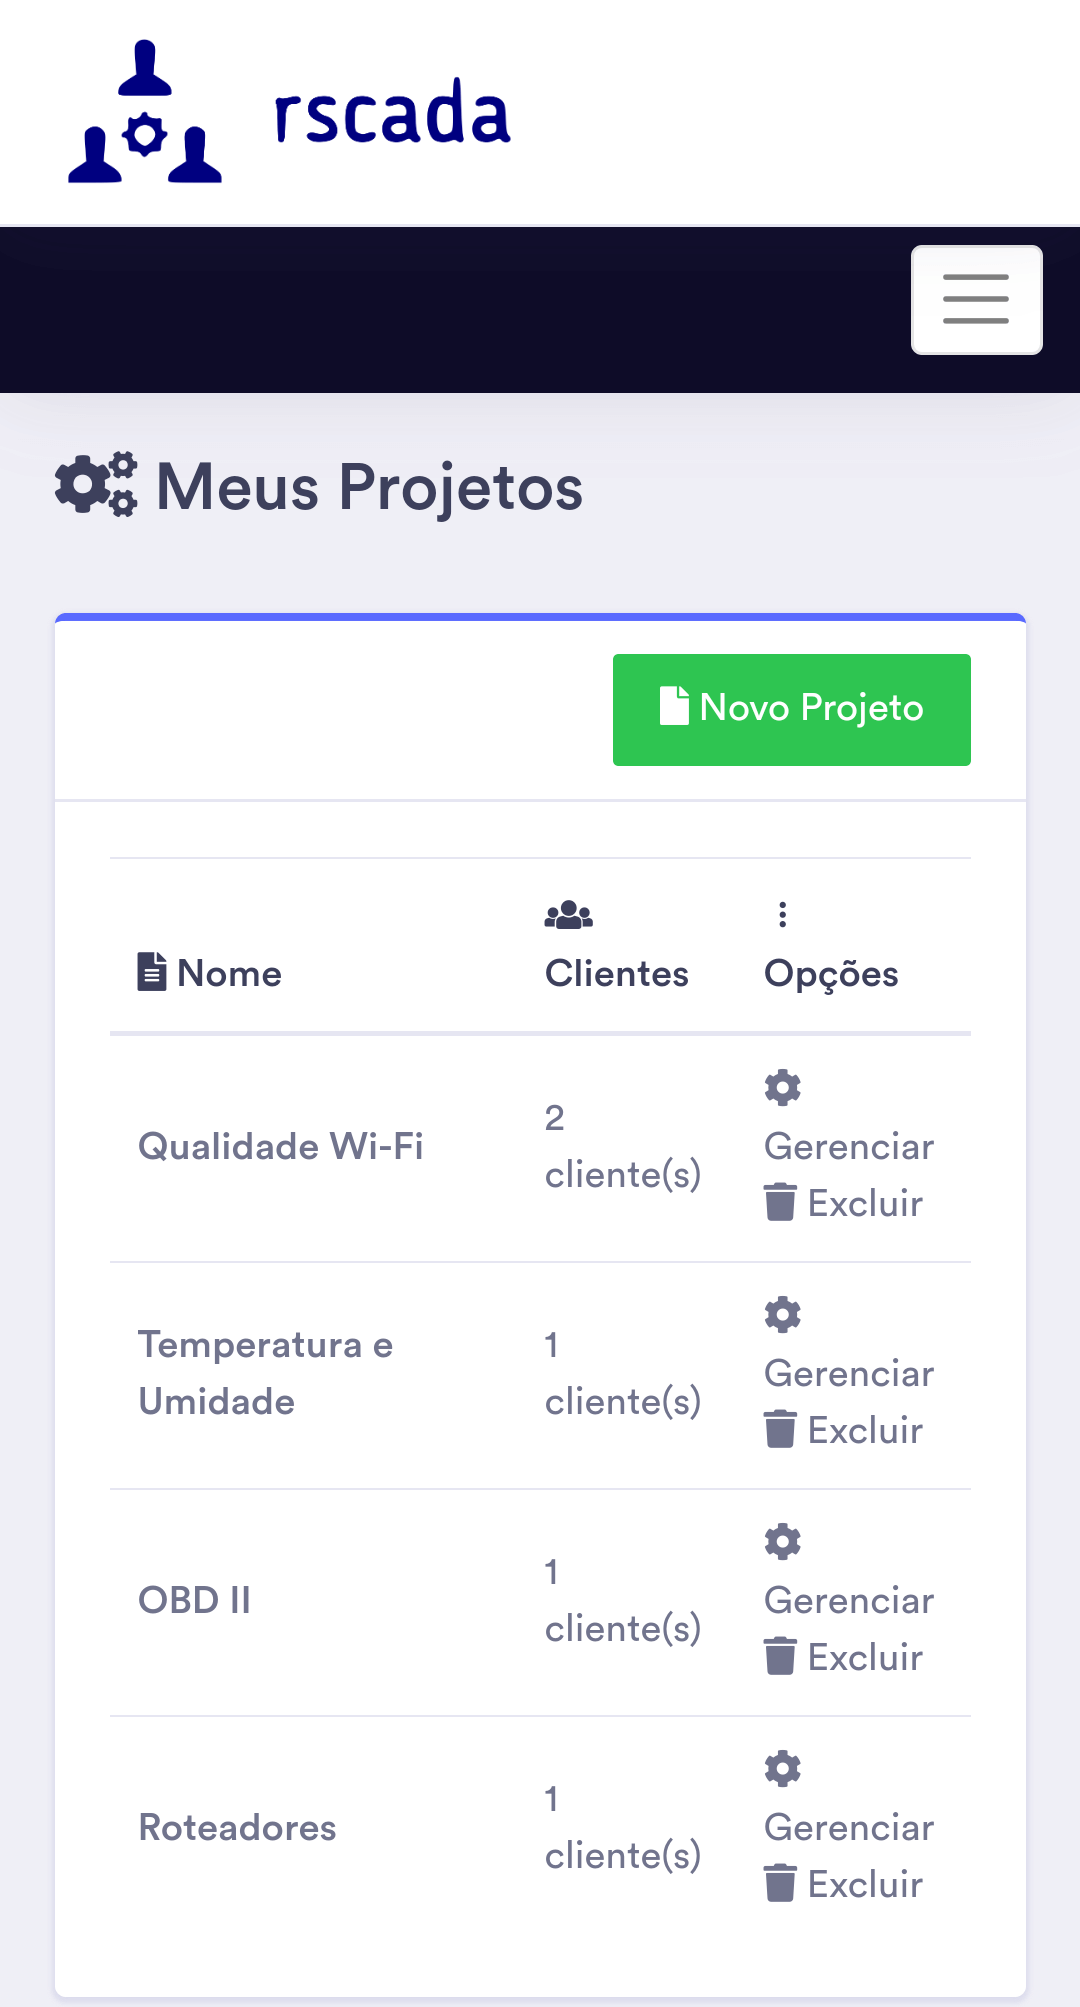
\includegraphics[width=7cm]{figuras/rscada-smartphone.png}}
		}{
			\Fonte{O autor}
		}	
    	\end{figure}
    	
\section{Criação de novos projetos}
\label{sec:criacao-projetos}
Ao clicar no botão Novo Projeto, o usuário é redirecionado à uma página solicitando o nome que se deseja para ele, conforme apresentado na Figura \ref{fig:figura-rscada-4}. Ao submeter o formulário é apresentada uma mensagem de sucesso, caso seja possível a criação dele, em seguida, encaminhado à página inicial do projeto, representado na Figura \ref{fig:figura-rscada-novo}. 

        \begin{figure}[!h]
		\Caption{\label{fig:figura-rscada-4} Página de cadastro de novos Projetos.}
		%\centering
		\UFCfig{}{
			\fbox{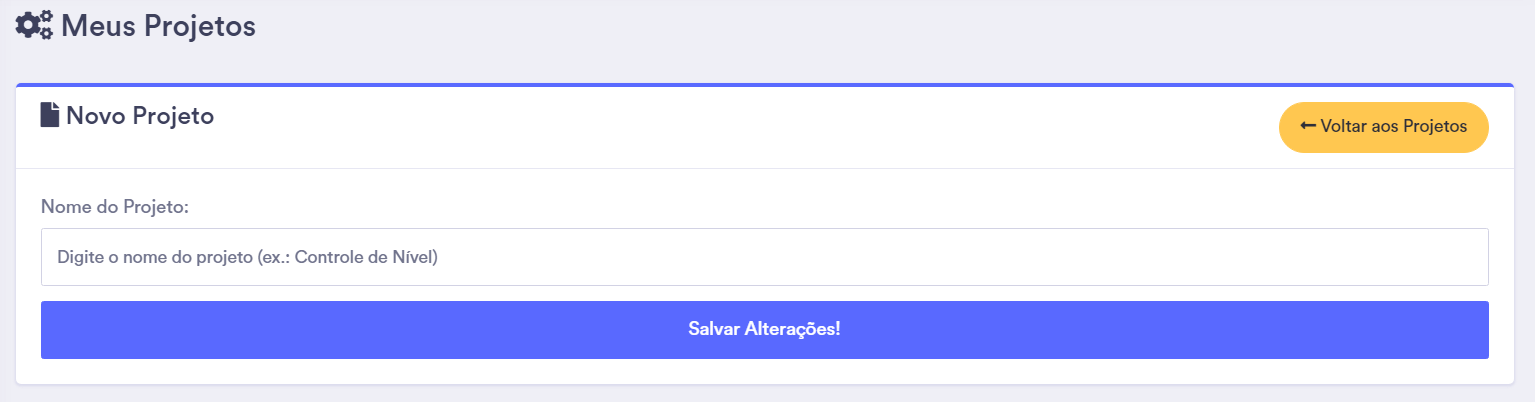
\includegraphics[width=15cm]{figuras/rscada-4.png}}
		}{
			\Fonte{O autor}
		}	
    	\end{figure}
    	
    	\begin{figure}[!h]
		\Caption{\label{fig:figura-rscada-novo} Página de gerenciamento de um novo projeto.}
		%\centering
		\UFCfig{}{
			\fbox{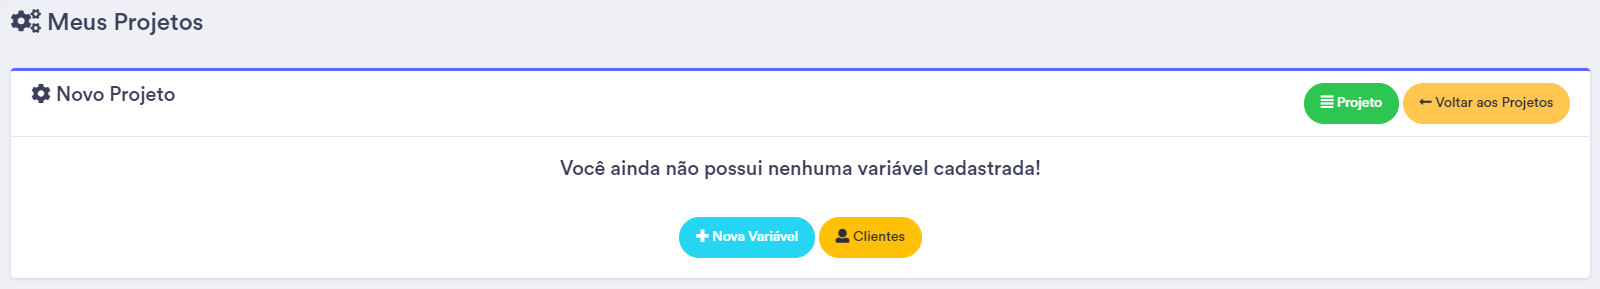
\includegraphics[width=15cm]{figuras/rscada-novo.png}}
		}{
			\Fonte{O autor}
		}	
    	\end{figure}

Nessa nova tela é apresentada uma mensagem de que não existe nenhuma variável cadastrada e há um reforço de cor no botão de criação para indicar a relevância dessa ação. Ao clicar no botão de Nova Variável, o usuário é redirecionado à uma tela ao qual poderá escolher o tipo pretendido, entre as citadas na seção \ref{sec:tipos-variaveis}, a variável iniciada por letra e minúscula, um nome que represente uma descrição à ela e a unidade correspondente caso exista. Na Figura \ref{fig:figura-rscada-6} é apresentada uma captura da tela de novas variáveis.

\newpage

        \begin{figure}[!h]
		\Caption{\label{fig:figura-rscada-6} Página de cadastro de novas Variáveis.}
		%\centering
		\UFCfig{}{
			\fbox{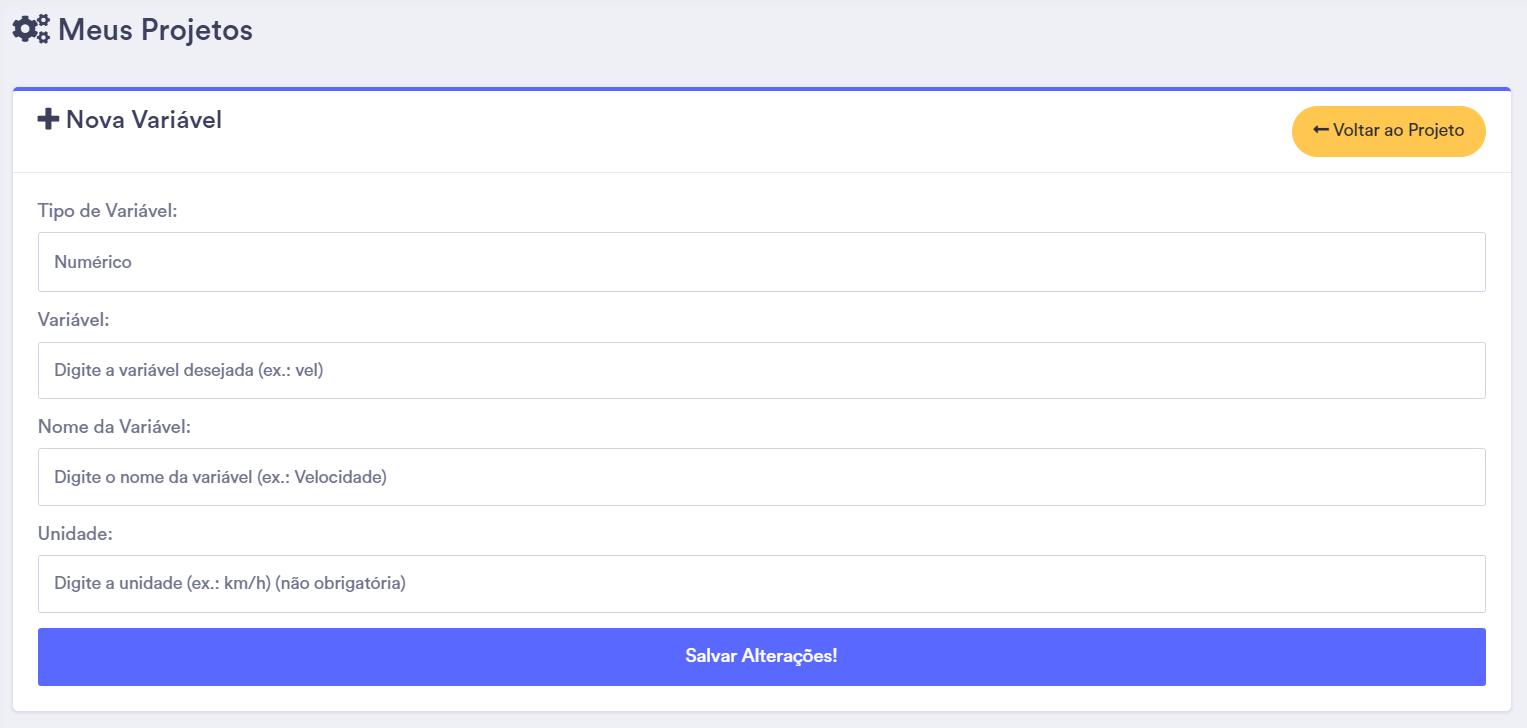
\includegraphics[width=15cm]{figuras/rscada-6.png}}
		}{
			\Fonte{O autor}
		}	
    	\end{figure}
    	
Quando submetido o formulário, é apresentada uma tela de sucesso caso a variável seja inserida no banco de dados e então, o usuário poderá gerenciar todas as variáveis já cadastradas no projeto com informação adicional sobre a quantidade de informações já inseridas no banco de dados para aquela variável específica, conforme representado na Figura \ref{fig:figura-rscada-variaveis} e coluna Registros. O cadastro de novas variáveis também pode ser feito diretamente no módulo de aquisição de dados, onde submetendo informações citando uma variável não cadastrada, o próprio módulo identificará o tipo dela e fará a submissão ao banco de dados. Este procedimento é feito para evitar a perda de informação, caso o desenvolvedor considere novas variáveis no dispositivo do processo e não tenha atualizado no sistema \gls{SCADA} ainda.

        \begin{figure}[!h]
		\Caption{\label{fig:figura-rscada-variaveis} Gerenciamento das variáveis cadastradas no projeto.}
		%\centering
		\UFCfig{}{
			\fbox{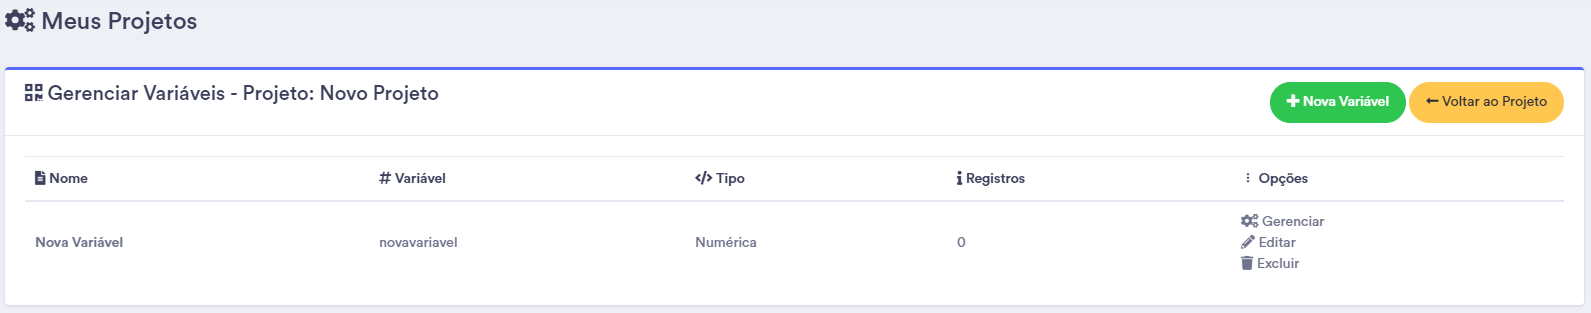
\includegraphics[width=15cm]{figuras/rscada-variaveis.png}}
		}{
			\Fonte{O autor}
		}	
    	\end{figure}

Com as variáveis já cadastradas no sistema, é oferecida a opção de criação de novos Objetos, detalhados na seção \ref{sec:projetos}, que quando clicado o botão, o usuário é direcionado à página ilustrada pela Figura \ref{fig:figura-rscada-7}. É solicitado o tipo do objeto, entre as opções já disponíveis na data de apresentação deste trabalho:

\begin{alineascomponto}
    \item Chave Binária: disponibiliza um botão que controla uma variável binária, à qual cada clique inverte seu valor, foi desenvolvida pensando em ser utilizada na função liga/desliga de alguma ação dentro do processo que seja necessário.
    \item Botão de Ação: disponibiliza um botão que pode oferecer o envio de um valor determinado em uma variável no instante em que for solicitado. Foi desenvolvido pensando em ser utilizado em funções que não sejam sustentadas, ou seja, tenha um único acionamento com período de duração determinado.
    \item Último Valor: disponibiliza um texto fixo com o último valor enviado pelo dispositivo da variável desejada no objeto. É dada a variação em relação ao valor imediatamente anterior à ele e o tempo que se passou desde o último envio.
    \item Gráfico de Linha: disponibiliza na tela um gráfico de linhas com uma série temporal das informações enviadas à variável escolhida. 
    \item Gráfico de Área: disponibiliza na tela um gráfico de área com uma série temporal das informações enviadas à variável escolhida.
    \item Gráfico de Barras: disponibiliza na tela um gráfico de barras com uma série temporal das informações enviadas à variável escolhida.
    \item Tabela de Informações: disponibiliza na tela uma tabela contendo uma quantidade dos últimos valores das informações enviadas à variável escolhida.
    \item Tabela de Eventos:  disponibiliza na tela uma tabela contendo os registros de alarmes e alertas sobre envio de informações que não estejam em acordo com o definido para a variável escolhida, representando também os alertas visuais que serão oferecidos ao operador quando ocorridas. Na Figura \ref{fig:figura-rscada-alarmes} são apresentados exemplos dos alarmes que são emitidos em tela para o Operador.
\end{alineascomponto}

Em seguida, são solicitados: Título, Descrição e Tamanho do Objeto, que servirão para apresentação da caixa gráfica quando inserida na interface do projeto. O Tamanho é uma seleção entre: Pequeno, Médio, Grande e Gigante, sendo respectivamente relacionado à largura ocupada da tela pelo Objeto, 25\%, 50\%, 75\% e 100\%.

\newpage

        \begin{figure}[!h]
		\Caption{\label{fig:figura-rscada-7} Página de cadastro de novos Objetos.}
		%\centering
		\UFCfig{}{
			\fbox{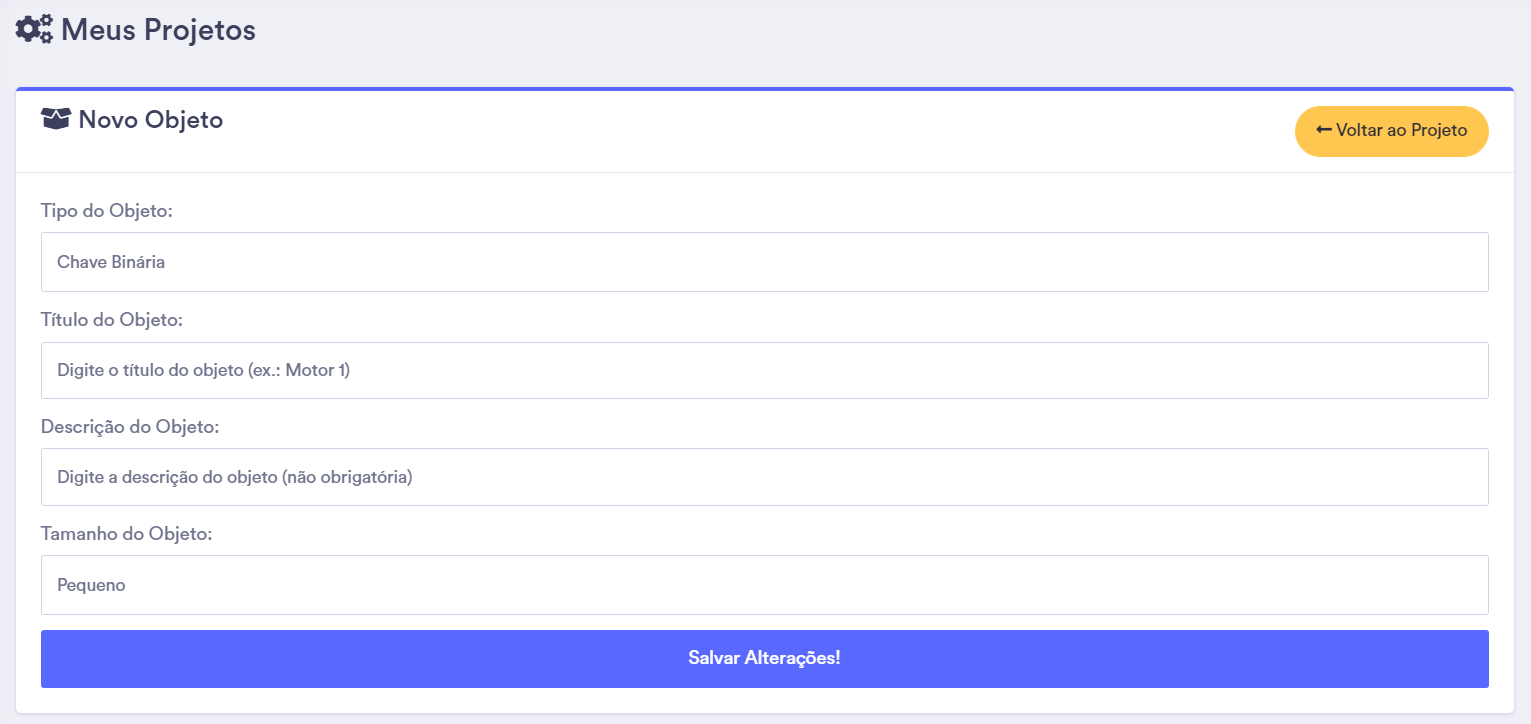
\includegraphics[width=15cm]{figuras/rscada-7.png}}
		}{
			\Fonte{O autor}
		}	
    	\end{figure}
    	
    	\begin{figure}[!h]
		\Caption{\label{fig:figura-rscada-alarmes} Alertas do sistema quando há uma não-conformidade da informação recebida.}
		%\centering
		\UFCfig{}{
			\fbox{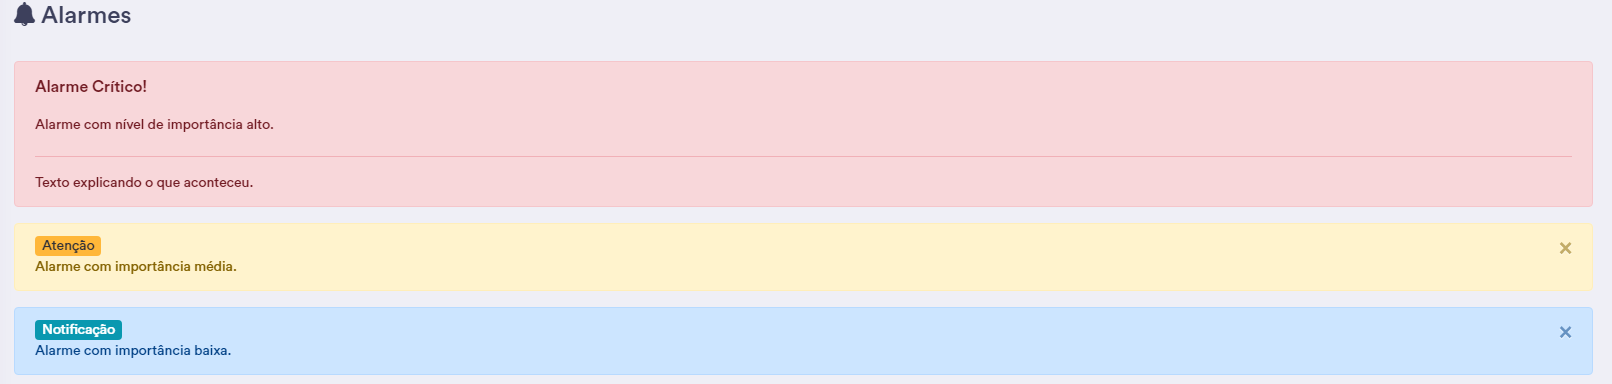
\includegraphics[width=15cm]{figuras/rscada-alarmes.png}}
		}{
			\Fonte{O autor}
		}	
    	\end{figure}
    	
Quando criado o objeto, é solicitada a edição dele para a determinação dos parâmetros referentes ao tipo específico escolhido, conforme apresentado na Figura \ref{fig:figura-rscada-10}. Na tela referente à edição do Objeto, é selecionada a variável que o objeto manipulará e a Janela de Tempo que seria a quantidade de pontos de informação à serem consideradas pelo sistema quando gerar o Objeto na interface de gerenciamento. Na Figura \ref{fig:figura-rscada-editar-objeto} é apresentado um exemplo de edição de um objeto do tipo Tabela de Informações em uma Nova Variável e Janela de Tempo de 5 minutos.
        
        \begin{figure}[!h]
		\Caption{\label{fig:figura-rscada-10} Objeto recém-criado.}
		%\centering
		\UFCfig{}{
			\fbox{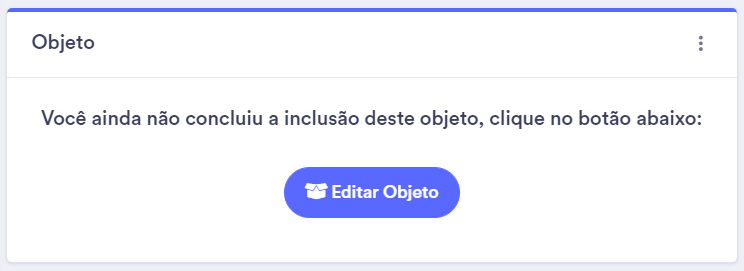
\includegraphics[width=12cm]{figuras/rscada-10.png}}
		}{
			\Fonte{O autor}
		}	
    	\end{figure}

    	\begin{figure}[!h]
		\Caption{\label{fig:figura-rscada-editar-objeto} Edição de objeto para determinação de parâmetros.}
		%\centering
		\UFCfig{}{
			\fbox{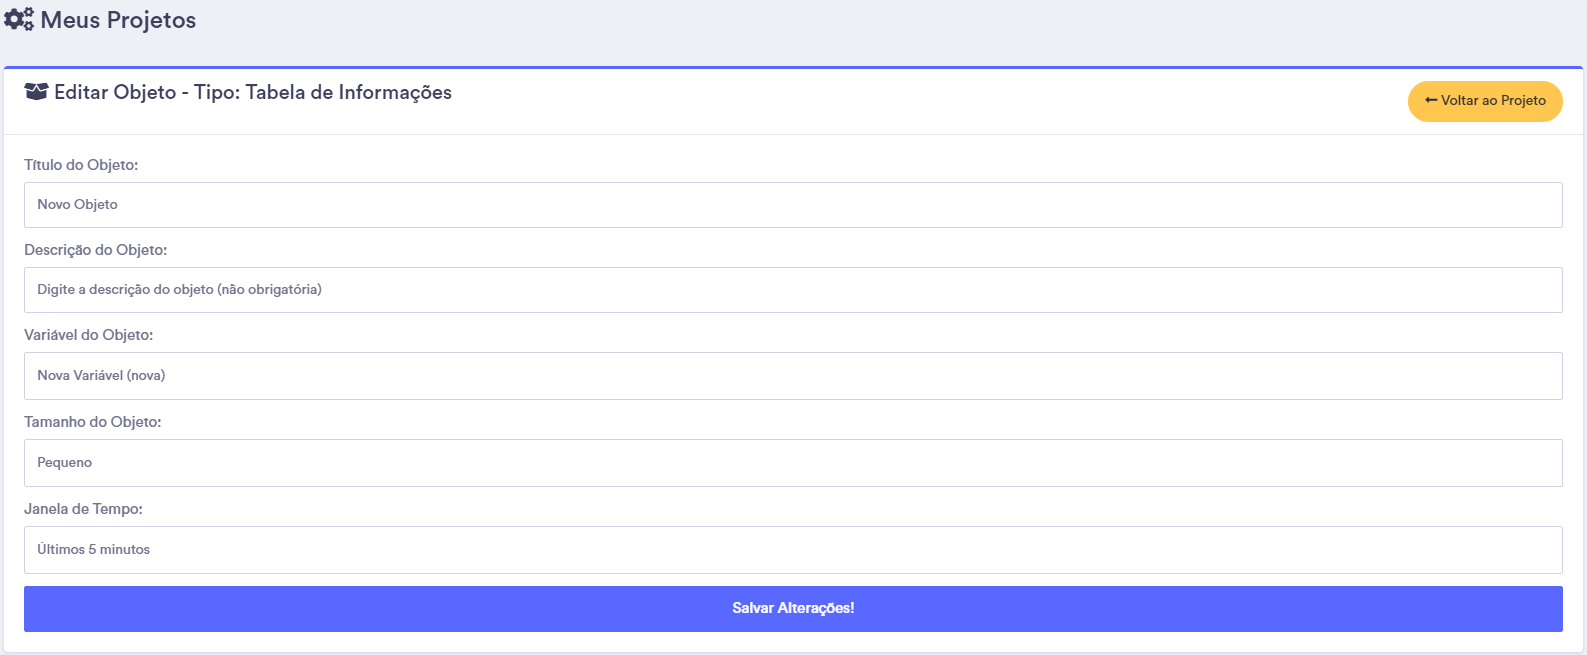
\includegraphics[width=15cm]{figuras/rscada-editar-objeto.png}}
		}{
			\Fonte{O autor}
		}	
    	\end{figure}

Após a organização dos Objetos e Variáveis da etapa anterior, deve ser feita a inclusão no menu Meus Clientes, dos operadores que utilizarão o projeto criado. A página Meus Clientes, disponibiliza um botão Novo Cliente, que após clicado, solicita dados do cliente, como: Nome, E-mail, Usuário e Senha que servirão para acesso do mesmo à interface de gerenciamento quando incluso no projeto. Na Figura \ref{fig:figura-rscada-novo-cliente} é apresentada a página de inclusão de novos clientes.

        \begin{figure}[!h]
		\Caption{\label{fig:figura-rscada-novo-cliente} Inserção de novo cliente ao sistema.}
		%\centering
		\UFCfig{}{
			\fbox{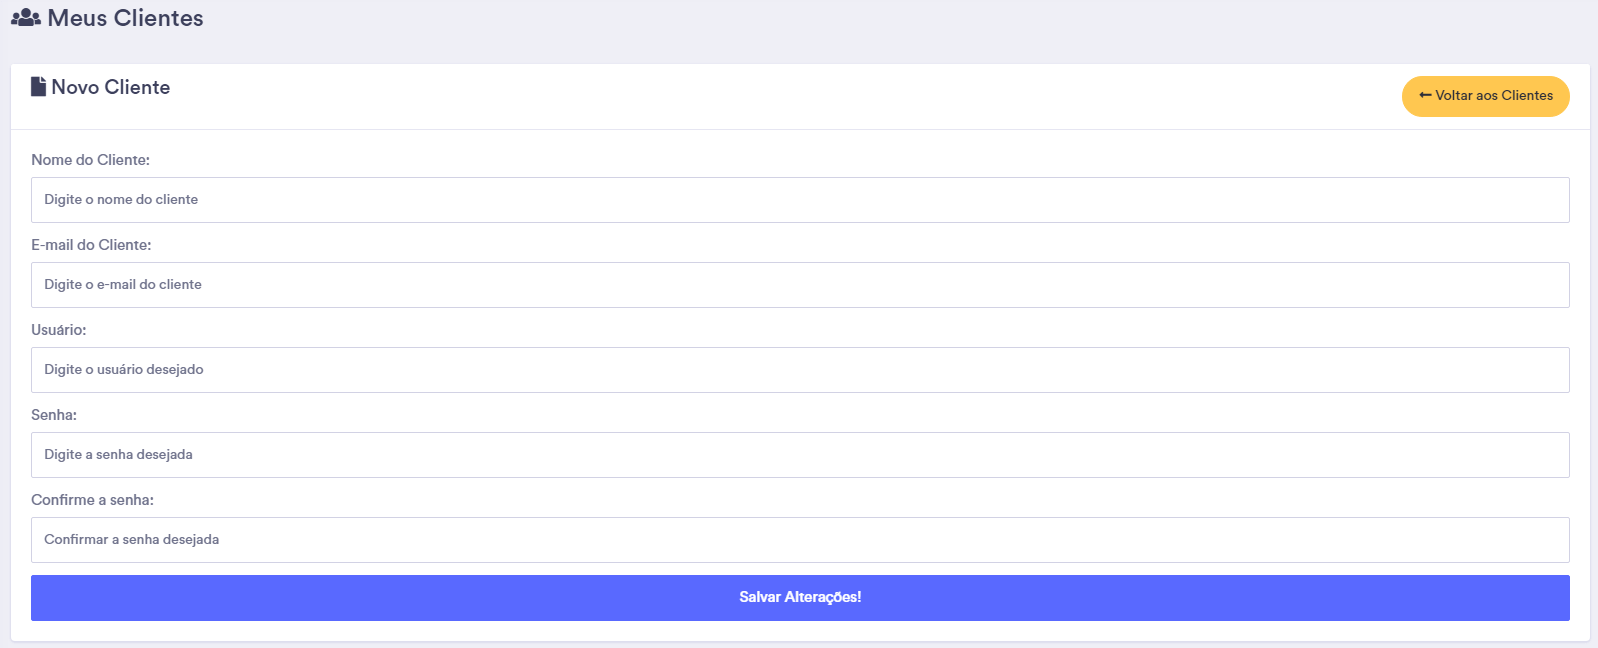
\includegraphics[width=15cm]{figuras/rscada-novo-cliente.png}}
		}{
			\Fonte{O autor}
		}	
    	\end{figure}
    	
\quad

\quad
    	
A submissão do formulário com os dados do cliente, desde que corretamente inseridos no banco de dados, resultará numa página com uma mensagem de sucesso e o usuário será direcionado à tela de gerenciamento de todos os clientes cadastrados no sistema, outras ações são disponíveis também nesta seção como o gerenciamento do cliente, alteração de seus dados de cadastro e a exclusão do mesmo, conforme apresentado na Figura \ref{fig:figura-rscada-clientes}.
    	
    	\begin{figure}[!h]
		\Caption{\label{fig:figura-rscada-clientes} Gerenciamento dos clientes cadastrados no sistema.}
		%\centering
		\UFCfig{}{
			\fbox{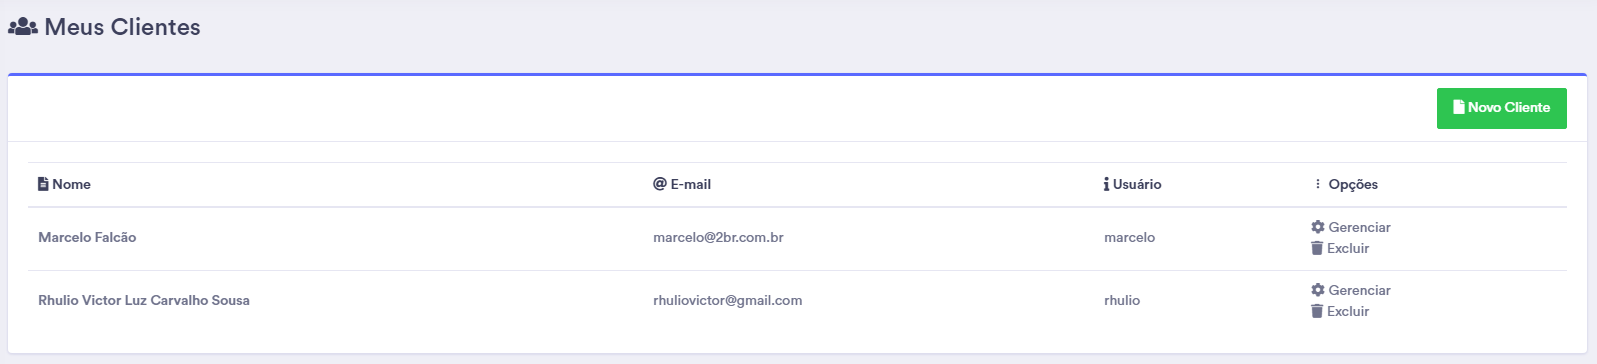
\includegraphics[width=15cm]{figuras/rscada-clientes.png}}
		}{
			\Fonte{O autor}
		}	
    	\end{figure}
    	
Após inserido um novo cliente, é possível fazer a associação do mesmo ao projeto criado anteriormente. Na Figura \ref{fig:figura-rscada-8} são apresentados detalhes de como é realizada esta ação no sistema. Desde que seja corretamente associado o cliente ao projeto e inserida esta informação no banco de dados, é retornada uma página de sucesso e o usuário é redirecionado à página de Clientes Associados. No qual podem ser verificados o \textit{Token} de acesso para envio de informações, nível do cliente e quantidade de informações enviadas por ele. Estão disponíveis também outras ferramentas, como: Editar a associação entre cliente e projeto e, a exclusão do mesmo, conforme a Figura \ref{fig:figura-rscada-9} que traz detalhes da tela.
    	
        \begin{figure}[!h]
		\Caption{\label{fig:figura-rscada-8} Associação de novo cliente ao projeto.}
		%\centering
		\UFCfig{}{
			\fbox{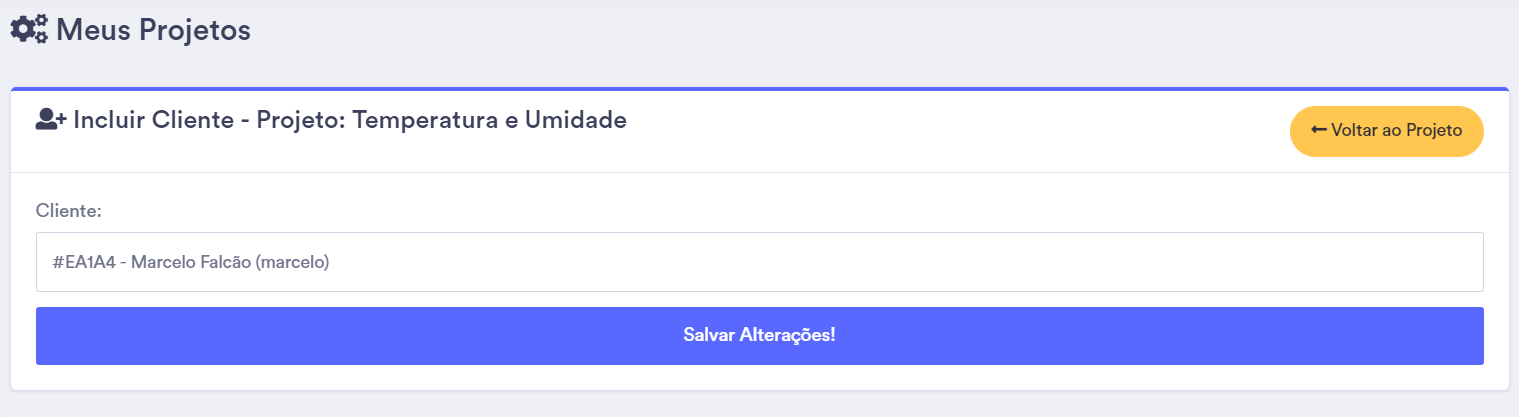
\includegraphics[width=15cm]{figuras/rscada-8.png}}
		}{
			\Fonte{O autor}
		}	
    	\end{figure}

        \begin{figure}[!h]
		\Caption{\label{fig:figura-rscada-9} Visão geral dos clientes cadastrados no projeto.}
		%\centering
		\UFCfig{}{
			\fbox{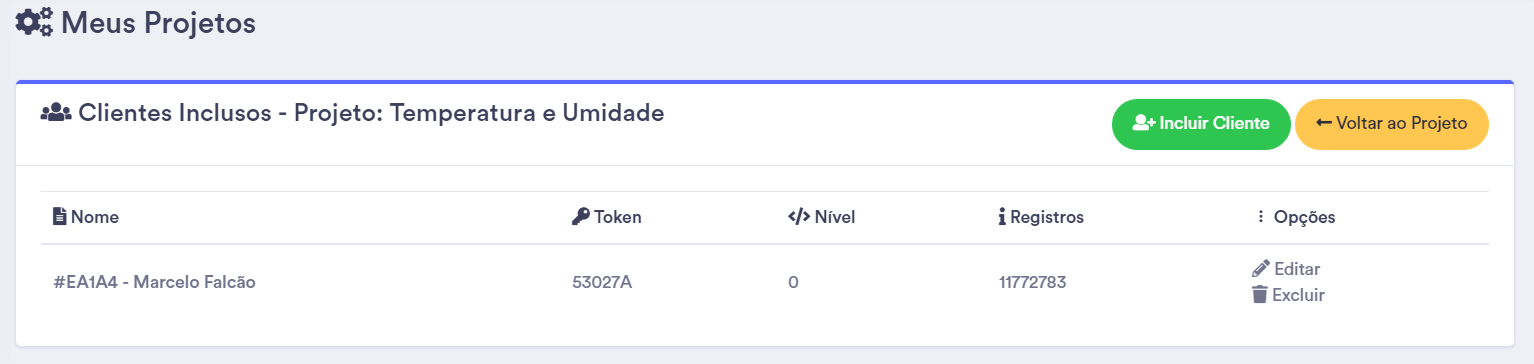
\includegraphics[width=15cm]{figuras/rscada-9.png}}
		}{
			\Fonte{O autor}
		}	
    	\end{figure}
    	
\section{Síntese}
\label{sec:sintese-rscada}

A abordagem utilizada neste Capítulo, pode ser sintetizada por um Diagrama de Caso de Uso, descrevendo a sequência e as unidades de interação com o sistema, disponível na Figura \ref{fig:figura-diagrama-uso}. Tendo sido detalhadas todas as funcionalidades propostas desenvolvidas, o capítulo seguinte traz uma aproximação do uso real deste sistema, com base em exemplos de diversas situações de utilização do mesmo. Os dois protocolos de aquisição de dados, \gls{MQTT} e \gls{HTTP}, são utilizados para demonstrar a facilidade de uso e a capacidade de integração do sistema.

        \begin{figure}[!h]
		\Caption{\label{fig:figura-diagrama-uso} Diagrama de caso de uso sintetizando os níveis de permissão do sistema.}
		%\centering
		\UFCfig{}{
			\fbox{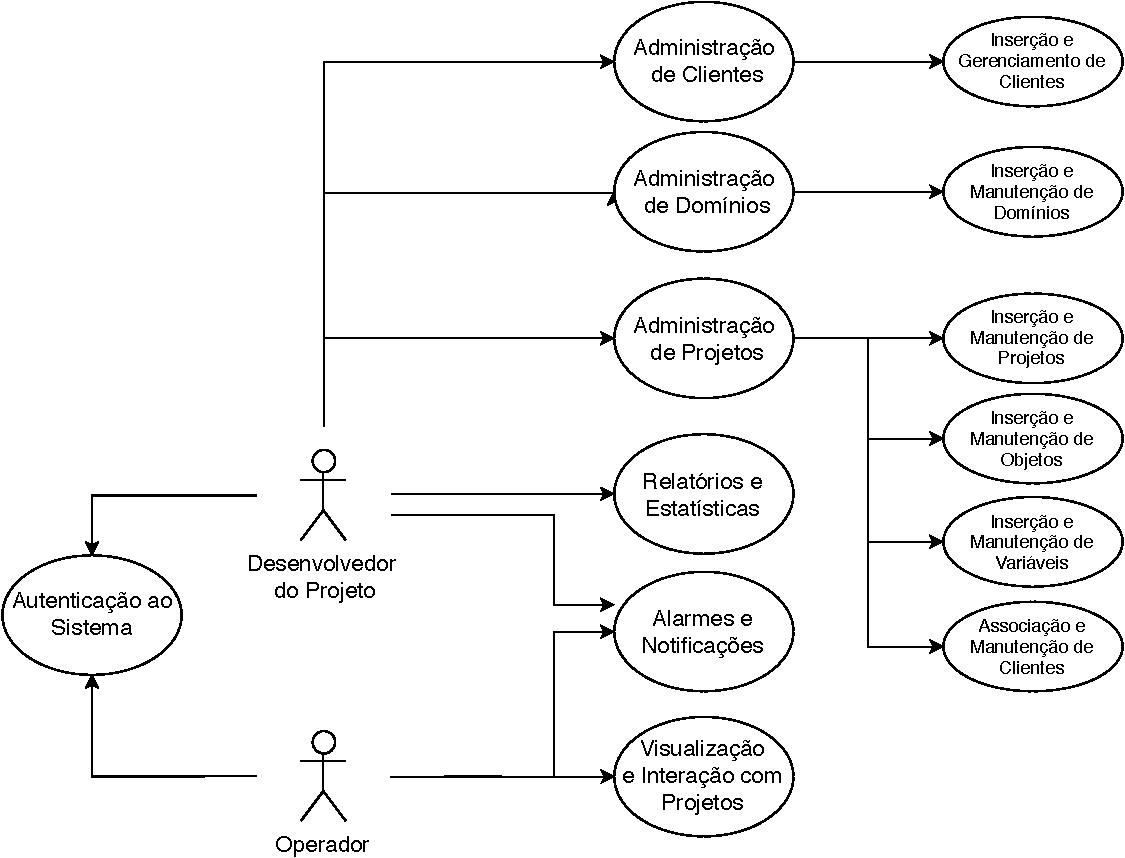
\includegraphics[width=15cm]{figuras/figura-diagrama-uso.pdf}}
		}{
			\Fonte{O autor}
		}	
    	\end{figure}
    	